% !TeX root = ../main.tex

\chapter{第二章}
\fancyhead[RH]{第二章\quad }
\section{第一节}

\begin{figure}[!htp]
    \centering
    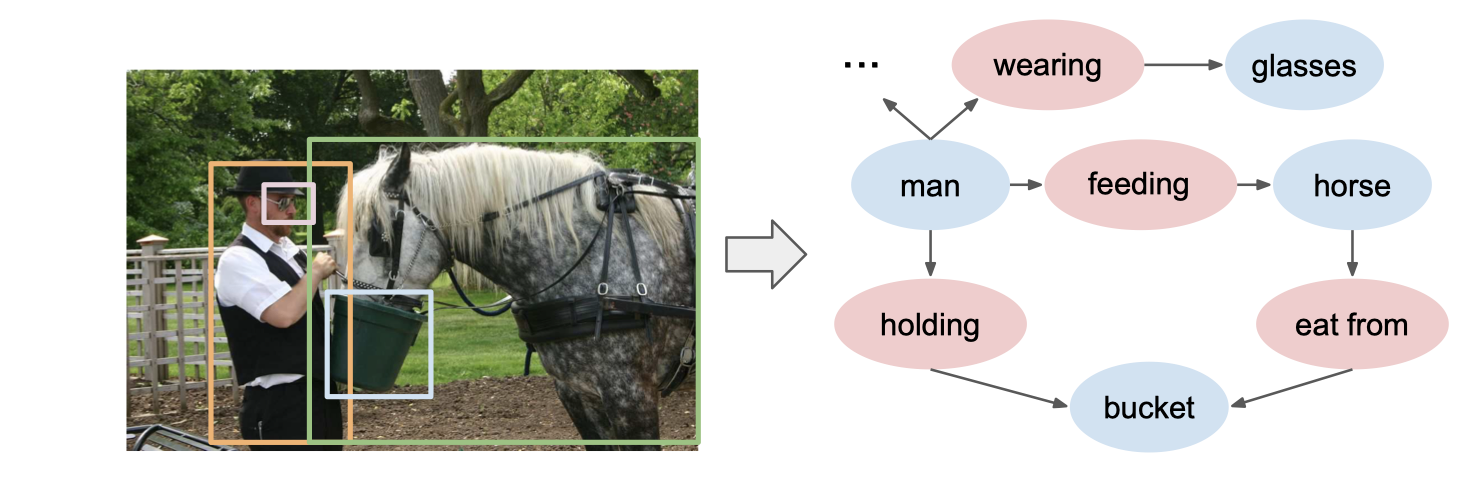
\includegraphics[width=1.0\textwidth]{figures/第二章/场景图示例.png} \\
    \bicaption[场景图示例]
    {场景图示例\cite{xu2017scene}}{Example of visual relationship dataset\cite{xu2017scene}}
   \label{场景图示例}
\end{figure}

\begin{equation}
    R(A, B) = 
    \begin{bmatrix}
        \partial A \cap \partial B & \partial A \cap B^0 & \partial A \cap B^- \\
        A^0 \cap \partial B & A^0 \cap b^0 & A^0 \cap B^- \\
        A^- \cap \partial B & A^- \cap B^0 & A^- \cap B^-
    \end{bmatrix}
\end{equation}



\section{第二节}



\section{本章小结}
